% =====================================================================
%  AVANT-PROPOS + CH. 1 — LE COFFRE EN UNE PAGE
% =====================================================================
\section*{Avant-propos — la place de ce livre}\label{sec:avantpropos}

\addcontentsline{toc}{section}{Avant-propos — la place de ce livre}

La spécification du protocole TRIADE dit \emph{ce qui doit être} ; ce livre dit
\emph{comment le tenir entre vos mains}. Il est le document complémentaire de la
spécification (v1.15 : l'édition courante est la v0.15.16) : il ne crée aucune règle,
n'amende aucune garde, n'invente aucun geste
— il porte la posture \emph{opératoire} du maître de cérémonie. Les mêmes vérités y
vivent, lues du côté de la main qui frappe la phrase, branche le média, recoupe le
checksum et décide, en dernier ressort, si l'ancien coffre peut mourir.

Trois lectures sont possibles, et elles sont toutes honnêtes. Le \textbf{maître de
cérémonie} lira dans l'ordre : le chapitre 1 pour voir l'ensemble, les chapitres 7 à 9
pour agir (cérémonies, runbook, mode dégradé), le reste en référence. L'\textbf{auditeur}
qui veut comprendre la chaîne lira les chapitres 2 à 6 — les trois générations, la
sentinelle, les gardes. Le \textbf{curieux pressé} lira le chapitre 1, le glossaire de
l'annexe B, et saura de quoi il parle. Aucune lecture ne exige les deux autres.

Une règle traverse tout le livre, énoncée une fois pour toutes : \textbf{en cas de
divergence entre ces pages et la spécification, la spécification fait foi} — et dans la
spécification, l'arbre signé \code{v06/I/} fait foi, parce qu'il est couvert par le
sceau de l'Intention : la signature Ed25519 de la clé hors-ligne du développeur. Ce
livre est daté, versionné, re-généré à chaque révision du protocole ; son absence
d'autorité n'est pas un défaut, c'est sa garantie.

\bigskip

\begin{center}
\large\bfseries Le coffre protège les secrets qui font vivre le dépôt.\\
Le sachet protège le coffre. La carte protège le sachet.\\
Vous protégez la carte.
\end{center}

\bigskip

\section{Le coffre en une page}\label{sec:unenpage}

\subsection{Ce que le coffre EST}

Le coffre-fort du protocole TRIADE est un \textbf{conteneur chiffré} qui centralise les
phrases maîtresses par projet — les secrets qui font vivre le dépôt : phrases de lignée,
phrases d'export, tout ce qui ne doit jamais vivre en clair sur une machine. Il est né
CF1 (D75), armé CF2 (D86), scellé CF3 (D121) : trois générations d'une même idée —
\emph{la clé qui déverrouille ne doit pas vivre entière là où le coffre dort}. Ce qui
n'a jamais changé d'une génération à l'autre : le contenu (le même JSON, la migration
ne traduit rien), la dérivation de la clé utilisateur (Argon2id aux planchers de la
carte : 65536 Kio, 3 itérations, parallélisme 1), le chiffrement (XChaCha20-Poly1305,
AAD = en-tête clair), la discipline \emph{fail-closed} (tout refus est nommé, aucune
écriture partielle, écriture atomique) et la discipline RAM (les clés vivotent en
\code{bytearray}, effacées au mieux de Python après usage).

\begin{figure}[htbp]
\centering
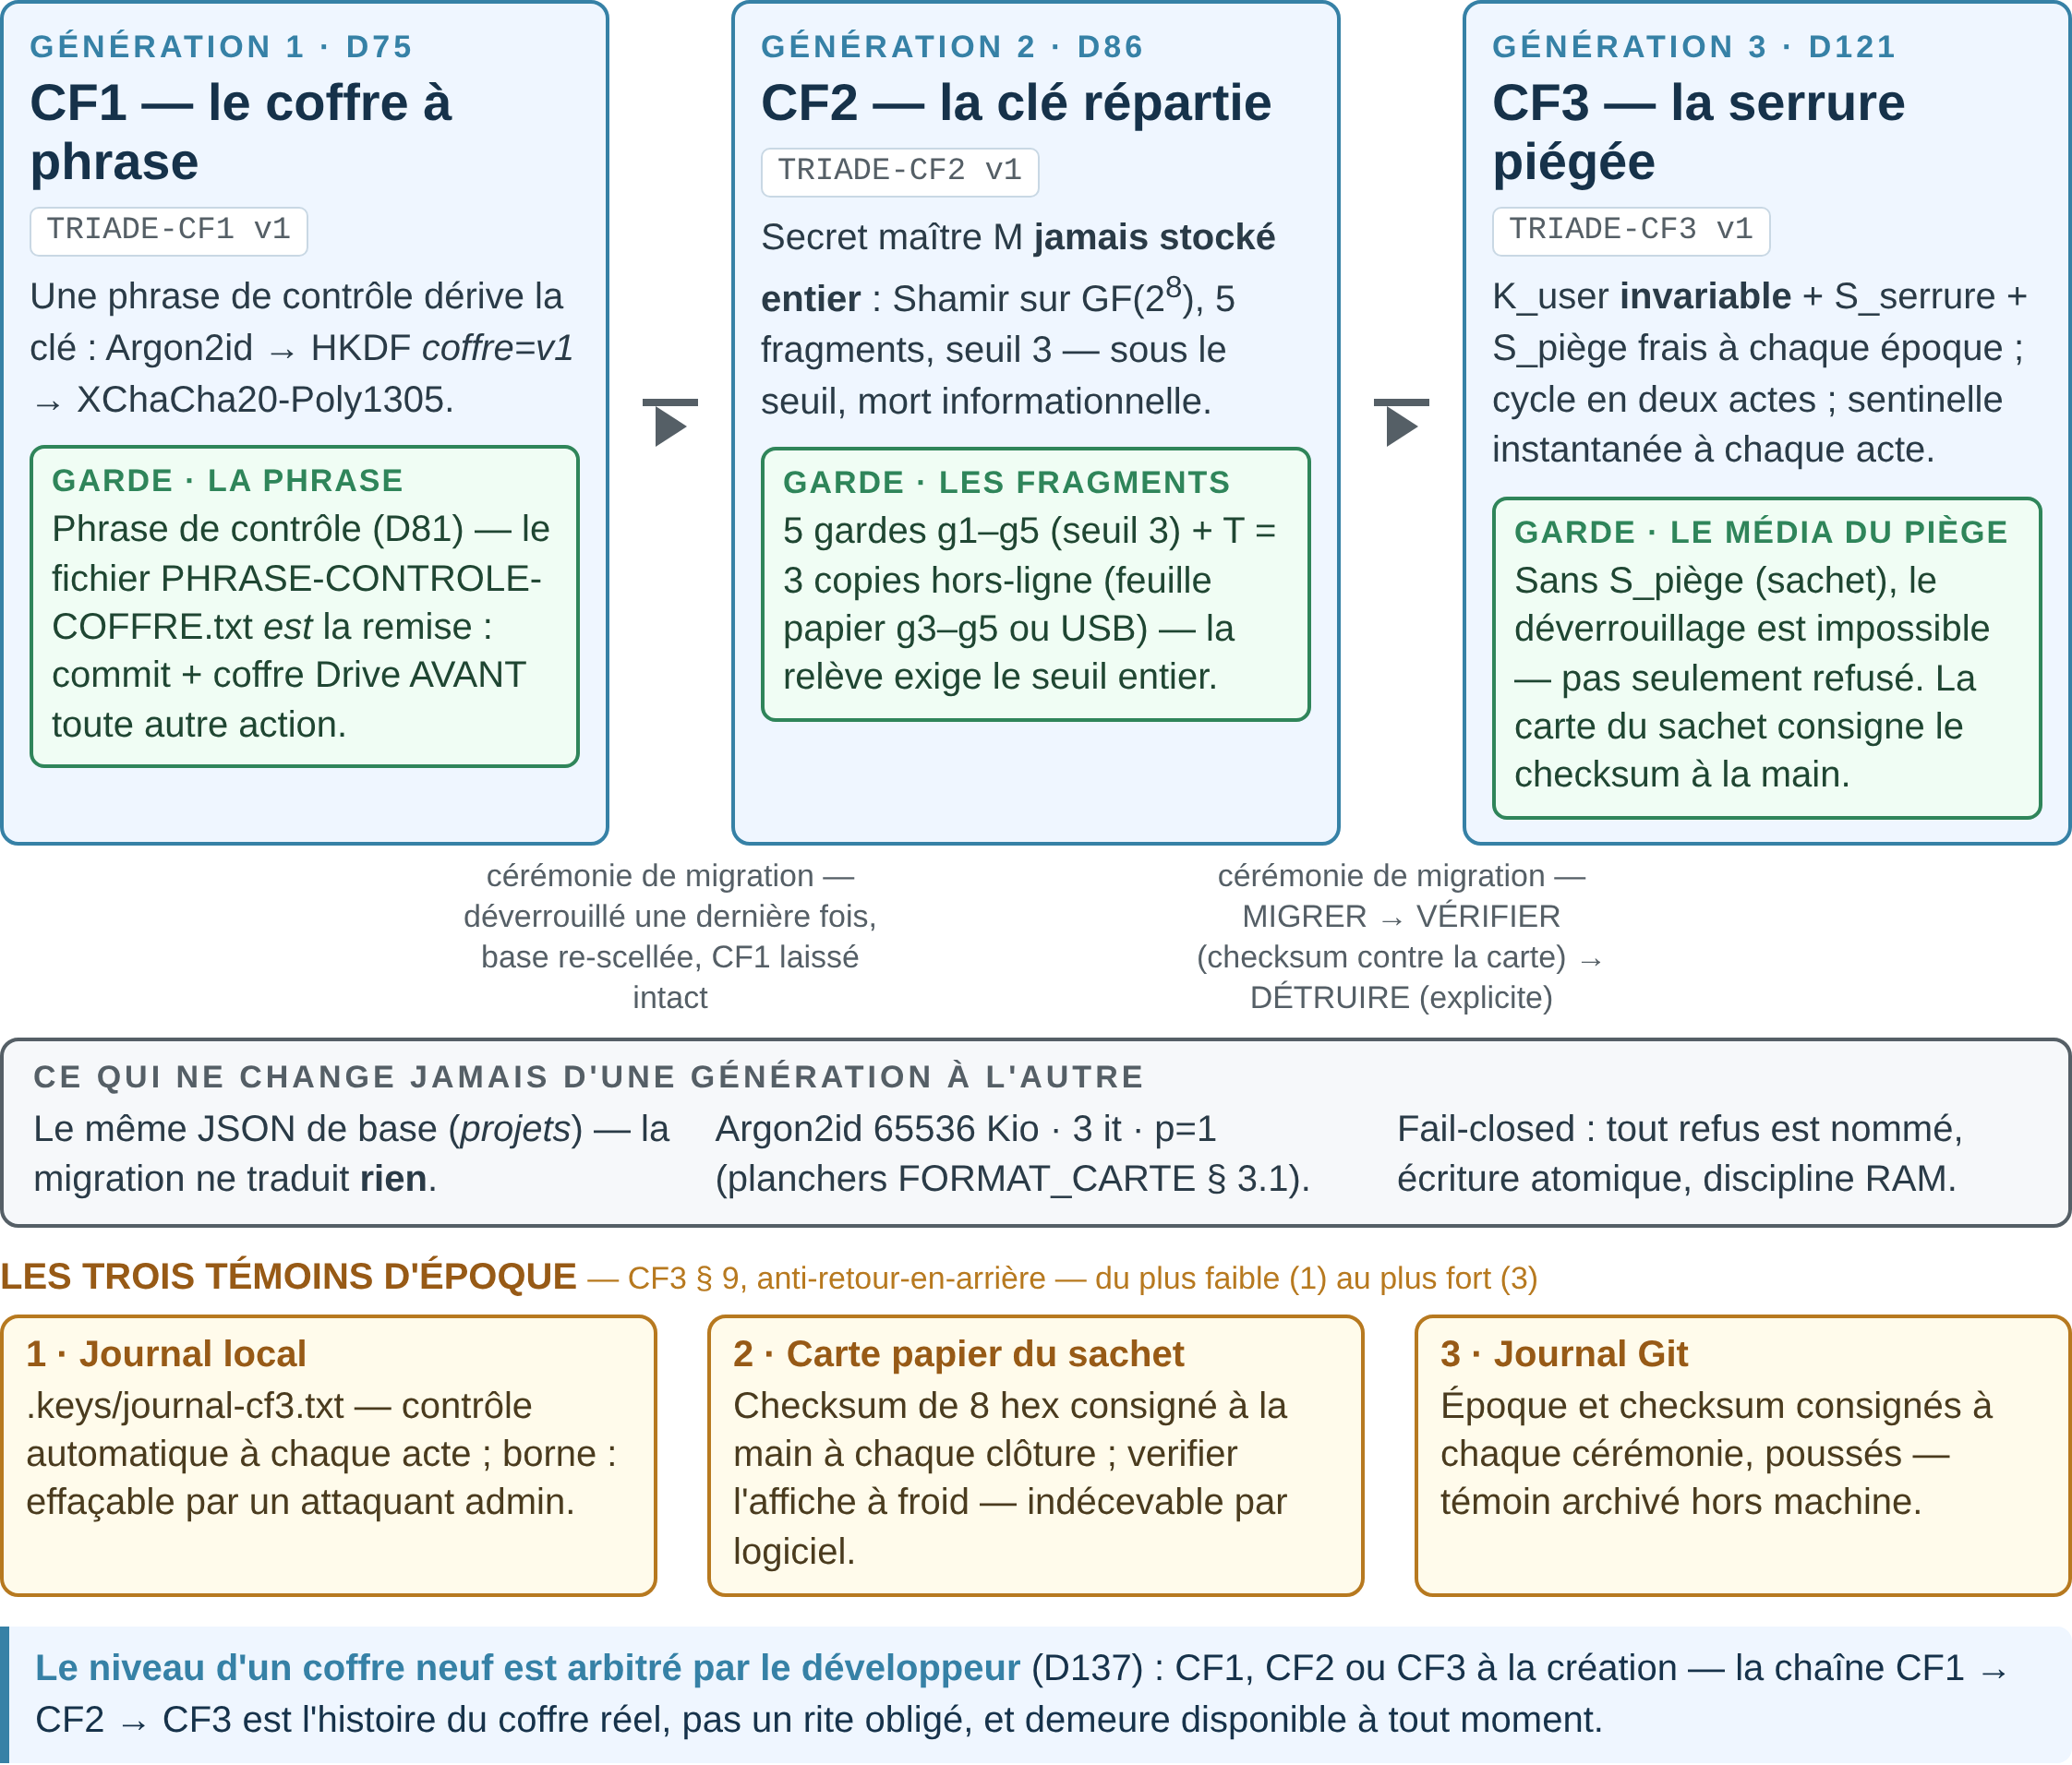
\includegraphics[width=\textwidth, max height=0.66\textheight]{chaine_cf}
\caption{La chaîne du coffre : trois générations, leurs gardes, les trois témoins
d'époque. Le niveau d'un coffre neuf est arbitré par le développeur (D137) — la
chaîne de migration est l'histoire du coffre réel, et demeure disponible à tout
moment.}
\label{fig:chaine}
\end{figure}

\subsection{Les trois générations, d'un coup d'œil}\label{sec:troisgenerations}

\begin{table}[htbp]
\centering\small
\caption{Les trois générations du coffre — d'un coup d'œil (le détail vit aux
chapitres 2 à 4).}
\label{tab:generations}
\begin{tabularx}{\textwidth}{@{}l Y Y Y@{}}
\toprule
 & \textbf{CF1} & \textbf{CF2} & \textbf{CF3} \\
\midrule
Née de & D75 (v0.5.1) & D86 (axe 2) & D121 (axe 4) \\
L'idée & une phrase suffit & la clé répartie vaut mieux & la serrure piégée
achève \\
Pour déverrouiller & la phrase & T fragments (seuil 3 sur 5) & la phrase ET le
piège d'époque égale \\
Ce qui peut manquer & la phrase (perdue = mort) & le seuil (sous 3 fragments =
mort informationnelle) & le média du piège (absent = acte impossible) \\
La garde vivante & la phrase sous séquestre 5/3 (amendé D223) & les gardes + la sentinelle & le sachet
+ la carte papier \\
Session & directe & directe, M effacé après l'acte & cycle en deux actes, brouillon
sous K\_session \\
Falsification prouvée & refus AEAD & refus AEAD + \code{verif} & destruction locale
+ PV — jamais le média \\
\bottomrule
\end{tabularx}
\end{table}

\subsection{Ce que le coffre N'EST PAS}\label{sec:pas}

Le coffre n'est pas un gestionnaire de mots de passe généraliste : il porte les
\emph{phrases maîtresses} du dépôt, pas vos comptes en ligne. Il n'est pas un coffre
d'artefacts : le dépôt git porte le code, la carte porte les empreintes — le coffre
porte ce qui \emph{ouvre} ces choses-là. Il n'est pas anonyme : chaque conteneur porte
son identité (magic, version, sel), chaque fragment son \code{coffre} (le sel, stable),
chaque piège son époque et son H\_projet. Et il n'est pas indulgent : une phrase
erronée est bénigne (réessai, délai croissant), mais une falsification \emph{prouvée}
détruit — la contrepartie qui rend le piège crédible (chapitre 4).

\subsection{Les trois règles du maître, avant tout le reste}\label{sec:troisregles}

\begin{enumerate}
\item \textbf{Jamais l'ancien avant le vert du neuf.} Chaque migration laisse l'ancien
conteneur intact jusqu'au verdict — CF1 est resté entier pendant la cérémonie CF2, CF2
est resté entier pendant la cérémonie CF3, et la destruction du CF2 reste un geste
explicite, après recoupement, sur machine froide de préférence.
\item \textbf{La phrase vit au séquestre, jamais au dépôt.} La garde active
est le séquestre D183 (D223) : cinq parts Shamir à seuil trois, les parts
inertes sous le seuil, la phrase en AUCUN dépôt — le dépôt est PUBLIC
(D220). La remise est la cérémonie de reconstitution à froid : trois parts
assemblées hors-ligne, la phrase reconstituée jamais écrite au dépôt,
l'usage transient détruit après le geste. Tout geste qui tenterait de
réécrire la phrase (ou son fichier) au dépôt est REFUSÉ avec son nom.
(La garde D81 — le fichier-remise commité — est l'histoire datée : la
phrase y demeure à vie, la rotation fut le remède ; cf. § \ref{sec:guarded81}.)
\item \textbf{Le sachet est individuel et il se garde comme un objet physique.} Un
média du piège par coffre ; les copies hors-ligne des fragments y vivent à côté des
pièges d'époque ; la carte papier y consigne les checksums à la main. Le sachet ne se
branche que pendant les actes qui l'exigent.
\end{enumerate}
